\chapter{Periodic orbits in chaotic systems}
\label{chap:orbits}

%% CONTRIBUTION
\small \paragraph{Contributions} This chapter is largely based on the following publication\footnote{with the following author contributions.
Conceptualisation: MK, PVC, EAP. Data curation: MK. Formal Analysis: MK. Methodology: MK. Visualisation: MK. Writing – original draft:
MK. Writing – review and editing: MK, PVC, EAP, TNP. The contributions of Peter, Adam and Tim are highly appreciated.}

\vspace{\baselineskip}
\indent M Klöwer, PV Coveney, EA Paxton, and TN Palmer, 2021.
\emph{On periodic orbits in chaotic systems simulated at low precision}, in preparation.
\vspace{\baselineskip}
\normalsize

\section{Introduction}

Once upon a time

\section{Methods}
\subsection{Wasserstein distance}
\label{sec:wasserstein}

The invariant measure of a chaotic dynamical system is estimated with histogram binning. To assess the agreement
of two histograms representing invariant measures (either simulated or analytical) we use the Wasserstein distance,
a metric that derives from the theory of optimal transport, with an $L^1$ cost. The Wasserstein distance $W_1(\mu,\nu)$
is defined as the least cost at which one can transport all probability mass from histogram $\mu$ to another histogram $\nu$,
where the cost to move mass $m$ from a bin at location $x$ to a bin at location $y$ is $m \vert x-y \vert$ \citep{Paxton2021,Villani2003}.
This gives a non-parametric method to compare probability distributions which accounts for both differences in the probabilities
of events as well as their separations in the underlying space, so that closeness in Wasserstein distance truly corresponds
to a natural notion of closeness between probability distributions \citep[Thm 7.12]{Villani2003}.

\subsection{An improved random number generator for uniformly distributed floats}
\label{sec:randfloat}

Conventional random number generation for a float $f$ from a uniform distribution $U(0,1)$
in $[0,1)$ uses the following technique: First, 10, 23, or 52 random bits (for Float16, Float32, or Float64, respectively)
from an unsigned integer are used to set the mantissa bits of floating-point one. This creates a floating-point
number that is uniformly distributed in $[1,2)$ as all float formats are uniformly distributed in that range. Second,
$1$ is subtracted to obtain a float in $[0,1)$, i.e. $f \sim U(1,2) - 1$. While this approach is fast, it is statistically
imperfect as the resulting distribution does not contain all floats in $[0,1)$ due to the rounding error introduced
by the subtraction. This technique only samples from every second float in $[\tfrac{1}{2},1)$, every fourth in
$[\tfrac{1}{4},\tfrac{1}{2})$ and so every $2n$-th float in $[2^{-n-1},2^{-n})$. Furthermore, the smallest positive
number that can be obtained is about $10^{-7}$ for Float32 and $10^{-16}$ for Float64. This is many orders of
magnitude larger than minpos, the smallest representable positive float, which is about $10^{-45}$, $10^{-324}$ for
Float32, Float64, respectively.

We therefore developed a statistically improved conversion from a random unsigned integer to a uniformly distributed
float in $[0,1)$. Counting the number of leading zeros $l$ of a random unsigned integer yields $l = 0$ at probability
$p = \tfrac{1}{2}$, $l=1$ at probability $p=\tfrac{1}{4}$ and $l = k$ at probability $p=2^{-k-1}$. These probabilities
correspond exactly to the share of power-2 exponents in the unit range $[0,1)$ for floats.
Consequently, we translate the number of leading zeros $l$  to the respective exponent bits and use the remaining
bits of the unsigned integers for the mantissa bits. The statistical flaws from the conventional conversion as presented
above are avoided, but for practical reasons the smallest float that can be sampled is about $10^{-20}$ for both Float32
and Float64. It is therefore practically impossible to sample a zero with this technique, just as the chance of obtaining a
zero in $[0,1)$ is effectively 0 for floats with 32 or 64 bit. For Float32, for example, we implement this technique as shown
in Listing \ref{lst:randfloat}, the implementations for Float16 and Float64 are similar. See our implementation in the Julia-package
\href{https://github.com/JuliaRandom/RandomNumbers.jl}{RandomNumbers.jl} for further details. The random number generation
for uniformly distributed floats is used throughout this study.

\begin{figure}[tbhp]
\begin{lstlisting}[language=JuliaLocal,label=lst:randfloat,caption={\textbf{An improved random number generator (RNG) for uniformly
distributed floats.} The Julia function \texttt{randfloat} takes \texttt{rng} as an argument for an RNG for 64-bit unsigned integers \texttt{UInt64}.
\texttt{\%} is the remainder after division, for unsigned integers effectively converting between unsigned integers by adding leading
zeros or discarding leading bits. \texttt{?} indicates a one-line if-clause. \texttt{\&} is the bitwise logical and-operation. \texttt{$\vert$}
is the bitwise logical or-operation.}]
function randfloat(rng::Random.AbstractRNG,::Type{Float32})

    # 64 random bits with generator rng
    ui = rand(rng,UInt64)

    # count leading zeros of random UInt64
    lz = leading_zeros(ui)

    # then convert leading zeros to exponent bits of Float32
    # e.g. 01111110, and bitshift to the right position via <<23
    e = ((126 - lz) % UInt32) << 23

    # reuse the last bits of ui for the 23 mantissa bits
    # unless the leading zeros reach into those for lz > 40
    ui = lz > 40 ? rand(rng,UInt64) : ui

    # ui % UInt32 drops the first 32 bits
    # & 0x007f_ffff sets non-mantissa bits to 0
    # e | then combines exponent and mantissa
    # and reinterpret the UInt32 as Float32
    return reinterpret(Float32,e | ((ui % UInt32) & 0x007f_ffff))
end
\end{lstlisting}
\end{figure}

\subsection{Monte Carlo orbit search}
\label{sec:orbit_search}



\subsection{Efficient orbit search with distributed computing}
\label{sec:distributed_orbit_search}

\section{Revisiting the generalised Bernoulli map}
\subsection{The special $\beta = 2$ case}
\subsection{Effects of stochastic rounding}

\section{Orbits in the Lorenz 1996 system}
\subsection{The Lorenz 1996 system}
\subsection{Longer orbits with more variables}
\subsection{More variables instead of higher precision}

\begin{figure}[tbhp]
	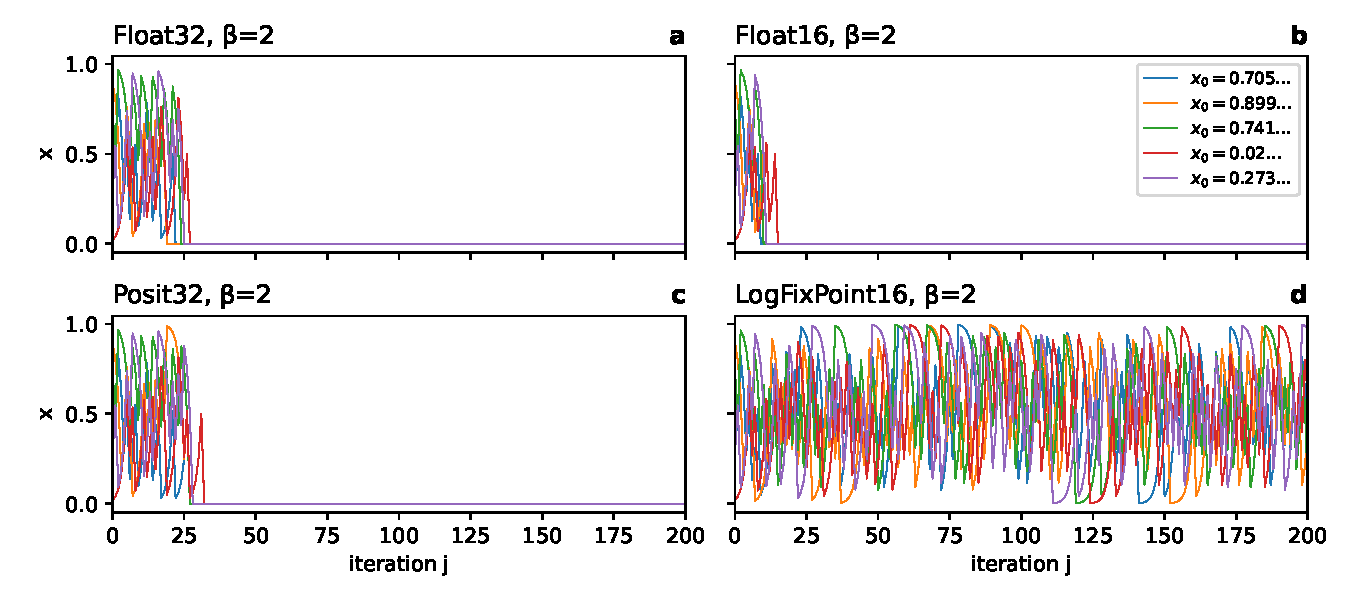
\includegraphics[width=1\textwidth]{Figures/orbits/beta2.pdf}
	\caption{\textbf{The Bernoulli map simulated with different number formats. a}
	Float32, \textbf{b} Float16, \textbf{c} Posit32, and \textbf{d} LogFixPoint16. The arithmetic operations in the
	Bernoulli map do not introduce rounding errors in \textbf{a}-\textbf{c}, only the initial conditions are subject
	to rounding, causing the attractor to collapse after a few iterations. However, the subtraction in the Bernoulli
	map causes rounding errors with logfix arithmetic in \textbf{d} that prevent the stalling at 0 from \textbf{a}-\textbf{c}.}
	\label{fig:orbits_beta2}
\end{figure}

\begin{figure}[tbhp]
	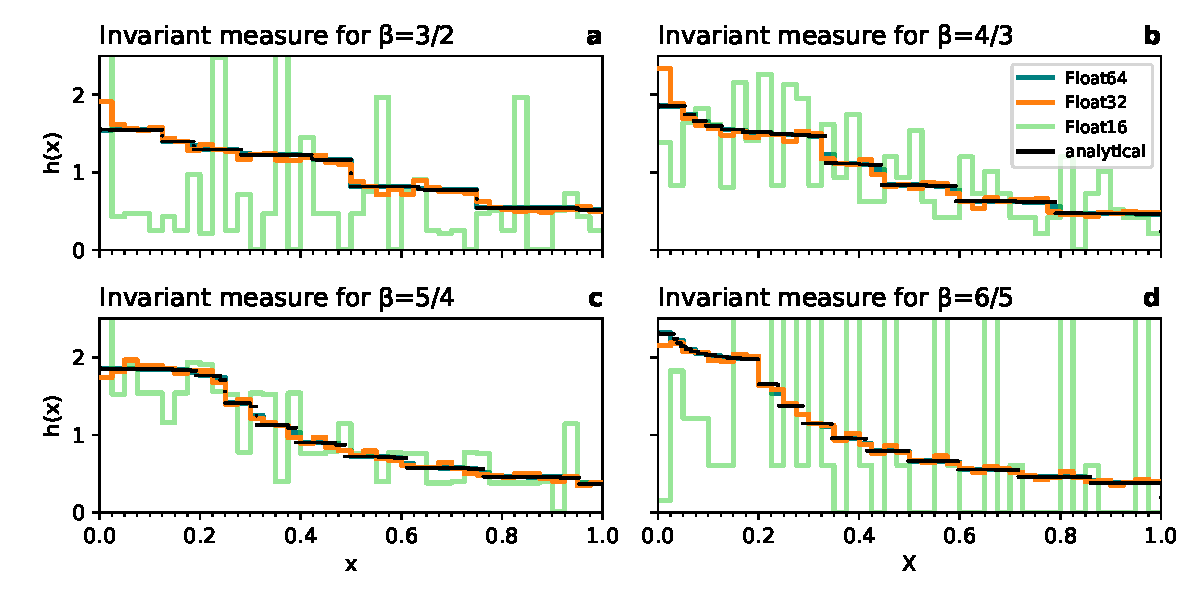
\includegraphics[width=1\textwidth]{Figures/orbits/inv_measures.pdf}
	\caption{\textbf{The invariant measure of the generalised Bernoulli map.}
	The generalised Bernoulli map is simulated with parameter \textbf{a} $\beta = \tfrac{3}{2}$,
	\textbf{b} $\beta = \tfrac{4}{3}$, \textbf{c} $\beta = \tfrac{5}{4}$, \textbf{d} $\beta = \tfrac{6}{5}$ and
	calculated with different number formats Float64, Float32 and Float16. The invariant measures of
	Float16 and Float32 are obtained from periodic orbits found by starting from 10,000 initial conditions
	$x_0 \in [0,1)$ chosen from a random uniform distribution. For Float64, long integrations (10,000 iterations,
	disregarding a spin-up of 5,000 iterations) of the Bernoulli map are used instead.
	Histograms use the bin width 0.025. The analytical invariant measure is not binned,
	which accounts for the discrepancy to Float64.}
	\label{fig:orbits_inv_measures}
\end{figure}

\begin{figure}[tbhp]
	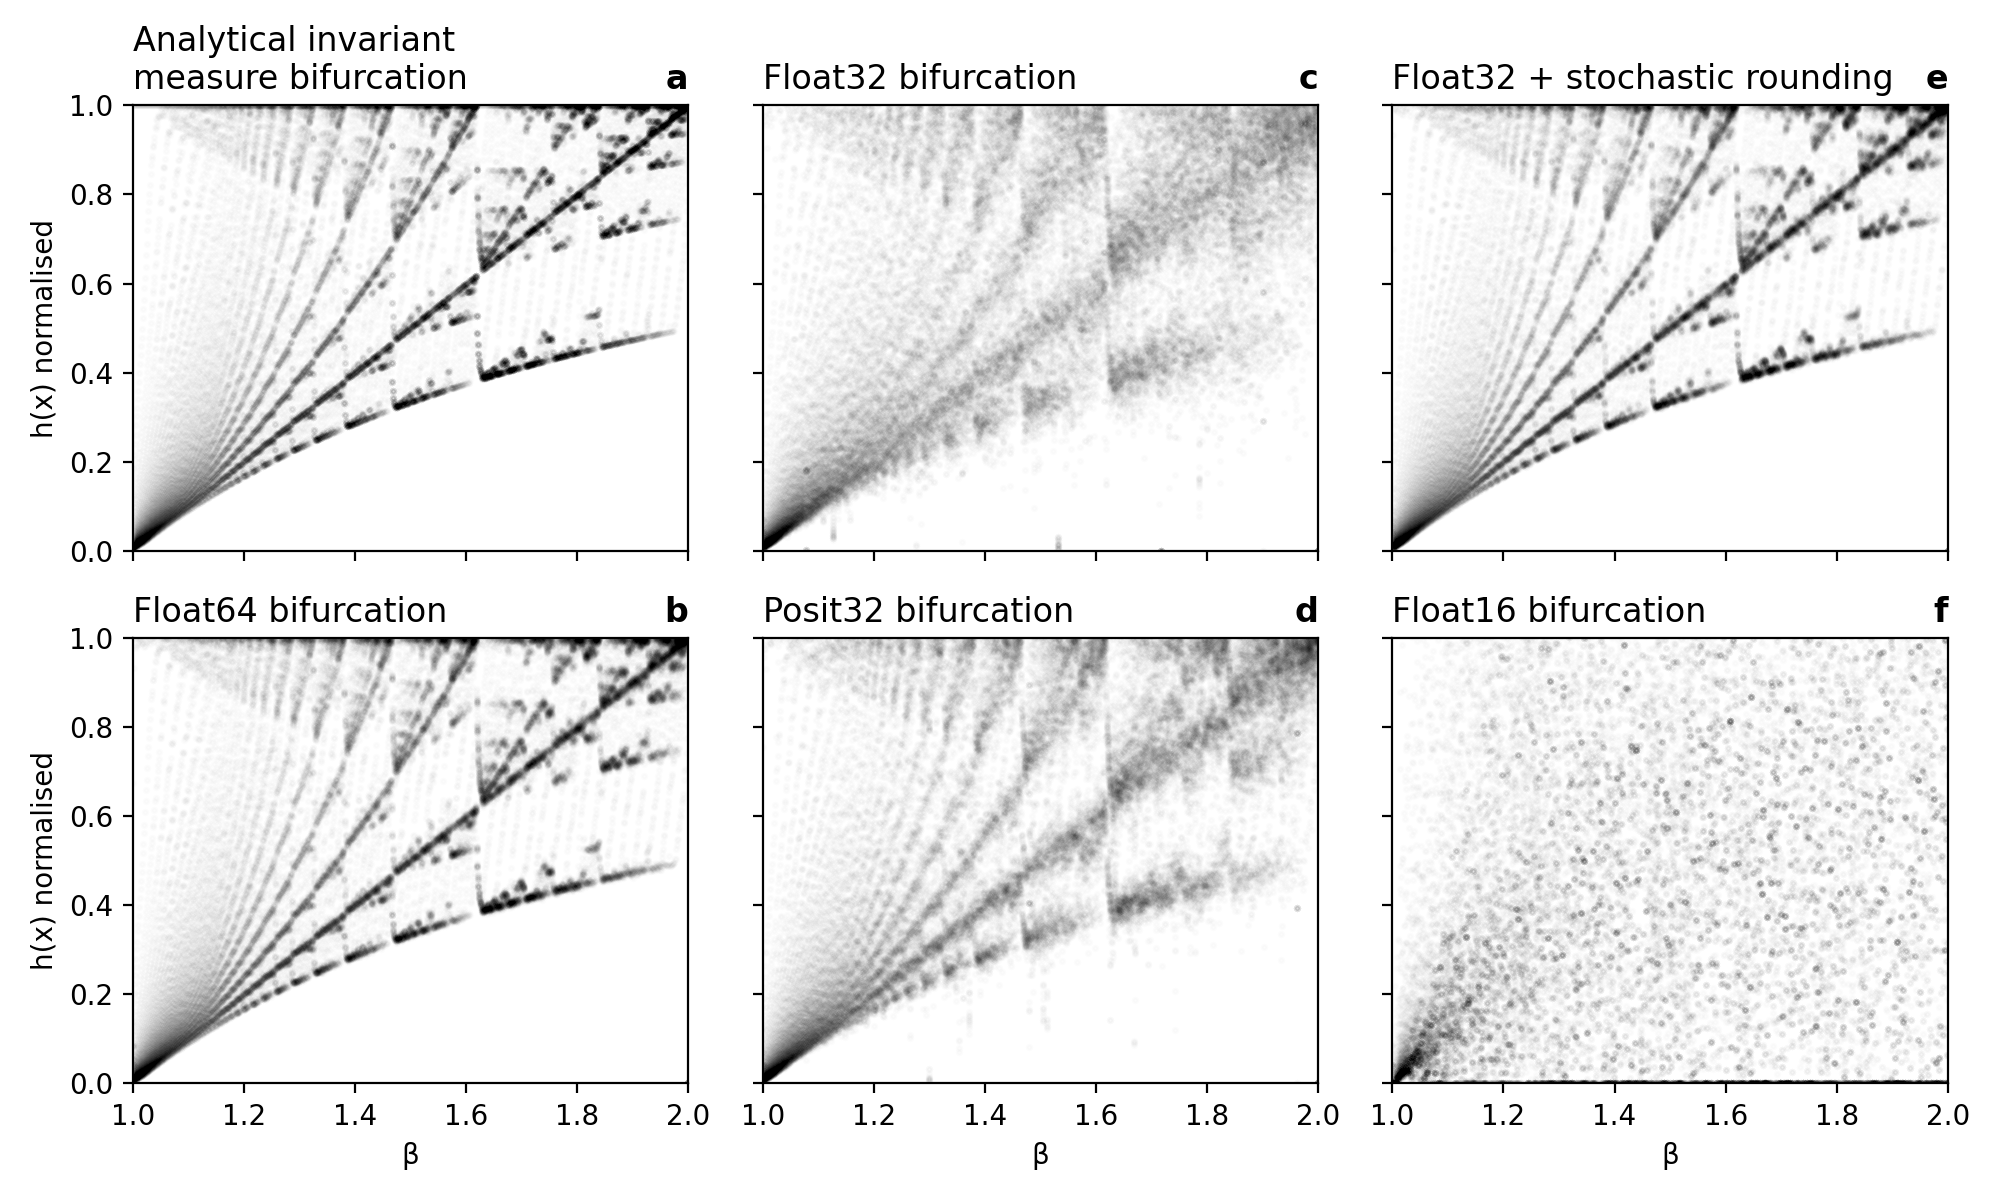
\includegraphics[width=1\textwidth]{Figures/orbits/bifurcation.png}
	\caption{\textbf{Bifurcation of the quantization levels corresponding to the invariant measures in
	the generalised Bernoulli map as simulated with various number formats. a}
	Analytical bifurcation $h_\beta(x)$ from the exact invariant measure, normalised by $\max(h_\beta(x))$,
	compared to the invariant measure by simulating the Bernoulli map with \textbf{b} Float64, \textbf{c} Float32,
	\textbf{d} Posit32, \textbf{e} Float32 and stochastic rounding, and \textbf{f} Float16.}
	\label{fig:orbits_bifurcation}
\end{figure}

\begin{figure}[tbhp]
	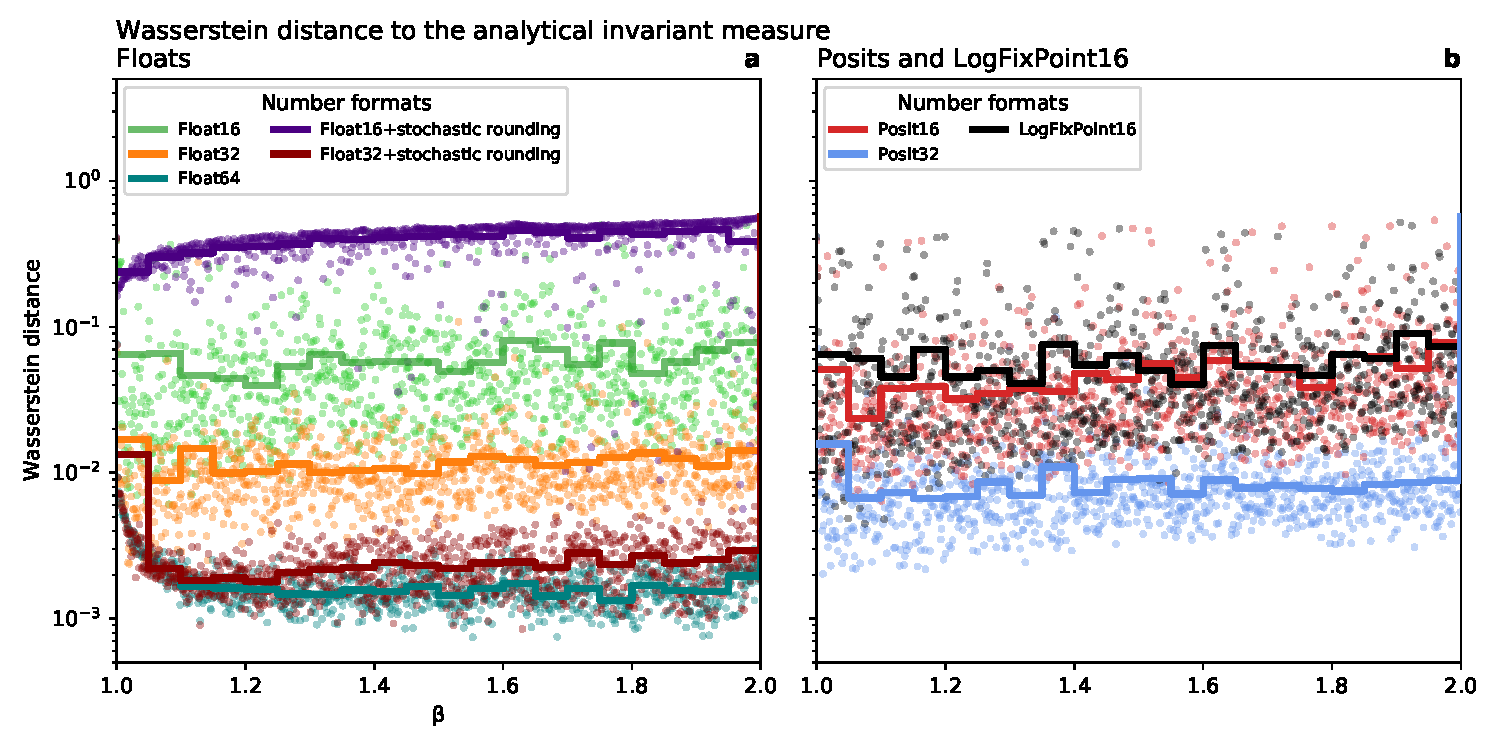
\includegraphics[width=1\textwidth]{Figures/orbits/wasserstein.pdf}
	\caption{\textbf{Agreement between the simulated and analytical invariant measures in the generalised
	Bernoulli map.} For all values except $\beta = 2$ a high precision number format yields a better agreement
	with the analytical Bernoulli map. Simulations using \textbf{a} Floats with and without stochastic rounding, 
	\textbf{b} Posits and LogFixPoint16. The Wasserstein distances are calculated for the invariant measures
	obtained from 1000 simulations for every value of $\beta$. Scatter points denote individual Wasserstein
	distances, solid lines indicate averages across a range of  as indicated by steps.}
	\label{fig:orbits_wasserstein}
\end{figure}

\begin{figure}[tbhp]
	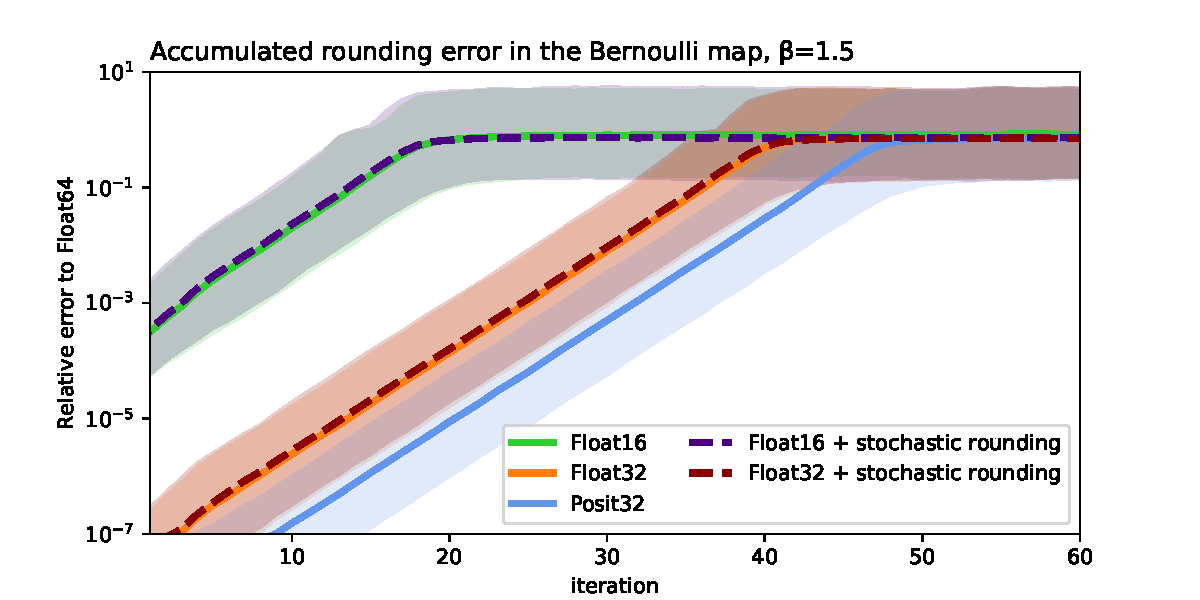
\includegraphics[width=1\textwidth]{Figures/orbits/error_growth.pdf}
	\caption{\textbf{Accumulated rounding error in the Bernoulli map.}
	Starting from 10,000 random initial conditions, the accumulated rounding error is the relative error of the
	given number format relative to a Float64 integration. Solid lines represent median errors across all
	initial conditions, shading the interdecile range. Other choices for the parameter $\beta$ of the generalised
	Bernoulli map yield a similar comparison between the number formats, but decreasing $\beta$ towards 1
	decreases the error growth for all formats similarly.}
	\label{fig:orbits_error_growth}
\end{figure}

\begin{figure}[tbhp]
	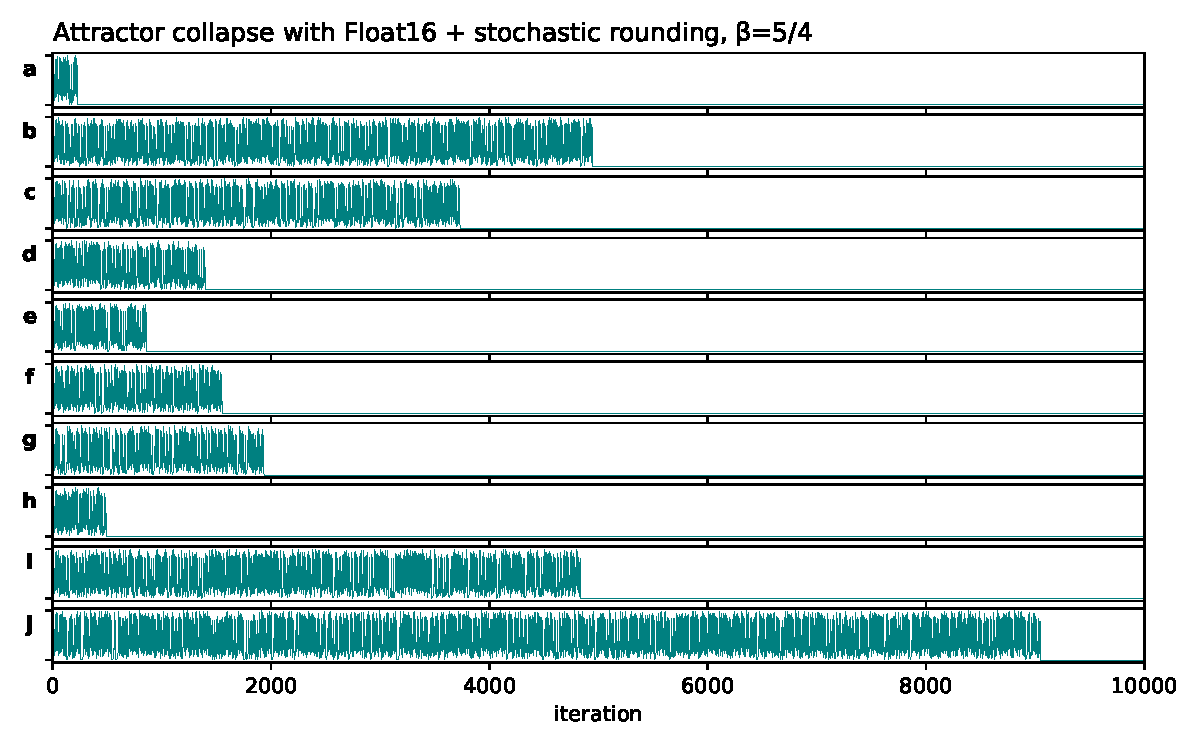
\includegraphics[width=1\textwidth]{Figures/orbits/attractor_collapse.pdf}
	\caption{\textbf{Attractor collapse of the generalised Bernoulli map with Float16 and stochastic roudning. a}-\textbf{j}
	Simulation of the Bernoulli starting from identical initial conditions and $\beta = 5/4$. Only the the
	state of the random number generator for stochastic rounding differs between \textbf{a}-\textbf{j}. After 10,000 iterations
	all simulations \textbf{a}-\textbf{j} stalled at the fixed-point 0 of the analytical attractor. The y-axes denote the value of
	$x_i$ in [0,1].}
	\label{fig:orbits_stochastic_collapse}
\end{figure}

\begin{figure}[tbhp]
	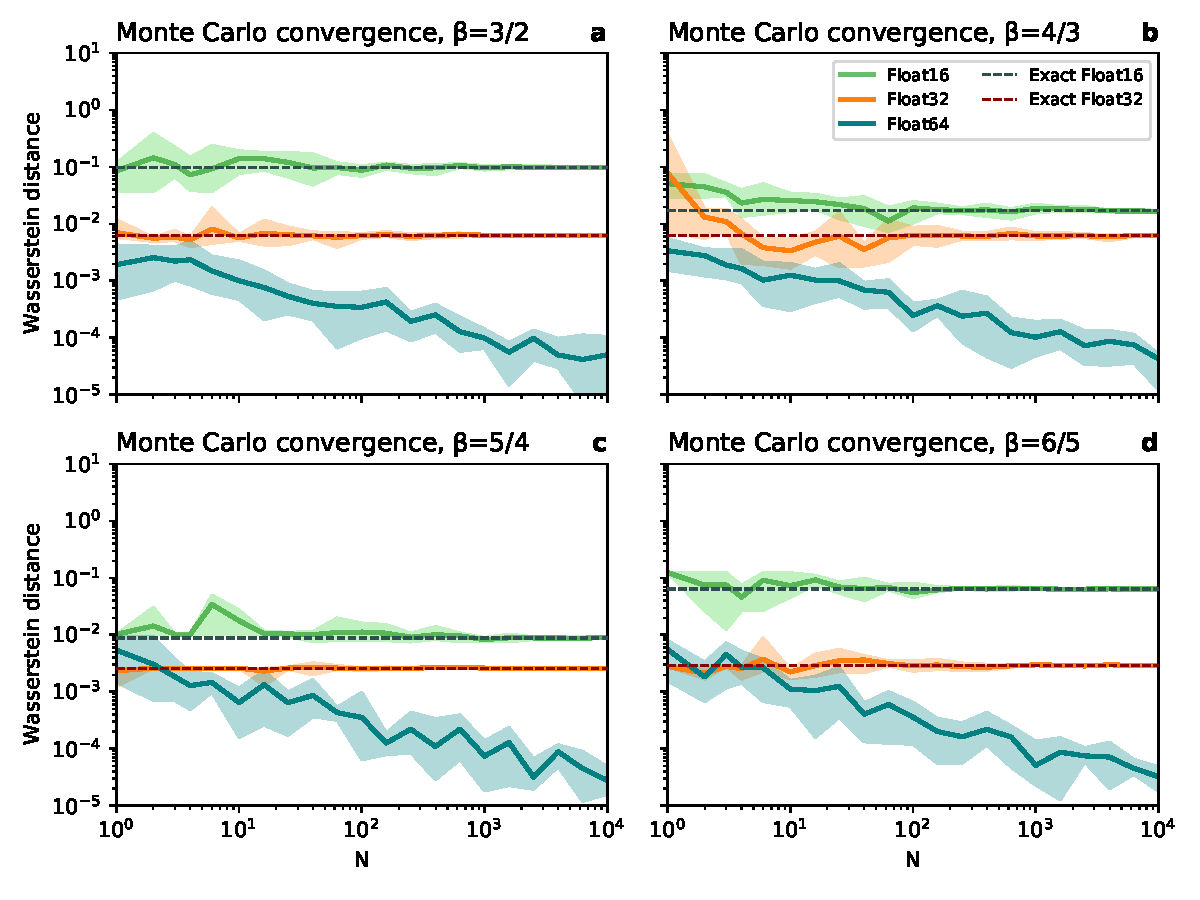
\includegraphics[width=1\textwidth]{Figures/orbits/convergence.pdf}
	\caption{\textbf{Convergence of the Monte Carlo sampling to estimate invariant measures.}
	The agreement between the analytical and simulated invariant measures (Figure \ref{fig:orbits_inv_measures})
	from $N$ random initial conditions uniformly distributed in $[0,1)$ are assessed with the Wasserstein distance
	(section \ref{sec:wasserstein}). About $N = 1000$ random initial conditions allow for a robust estimate of the
	invariant measure with Float16 and Float32, virtually identical with exact invariant measure obtained from
	computing all 15,360 Float16 and 1,065,353,216 Float32 numbers in $[0,1)$, respectively. The $\beta$ parameter
	of the generalised Bernoulli map is \textbf{a} $\beta = \tfrac{3}{2}$, \textbf{b} $\beta = \tfrac{4}{3}$,
	\textbf{c} $\beta = \tfrac{5}{4}$, and \textbf{d} $\beta = \tfrac{6}{5}$. Solid lines represent the mean and shading
	the min-max range.}
	\label{fig:orbits_convergence}
\end{figure}

\begin{figure}[tbhp]
	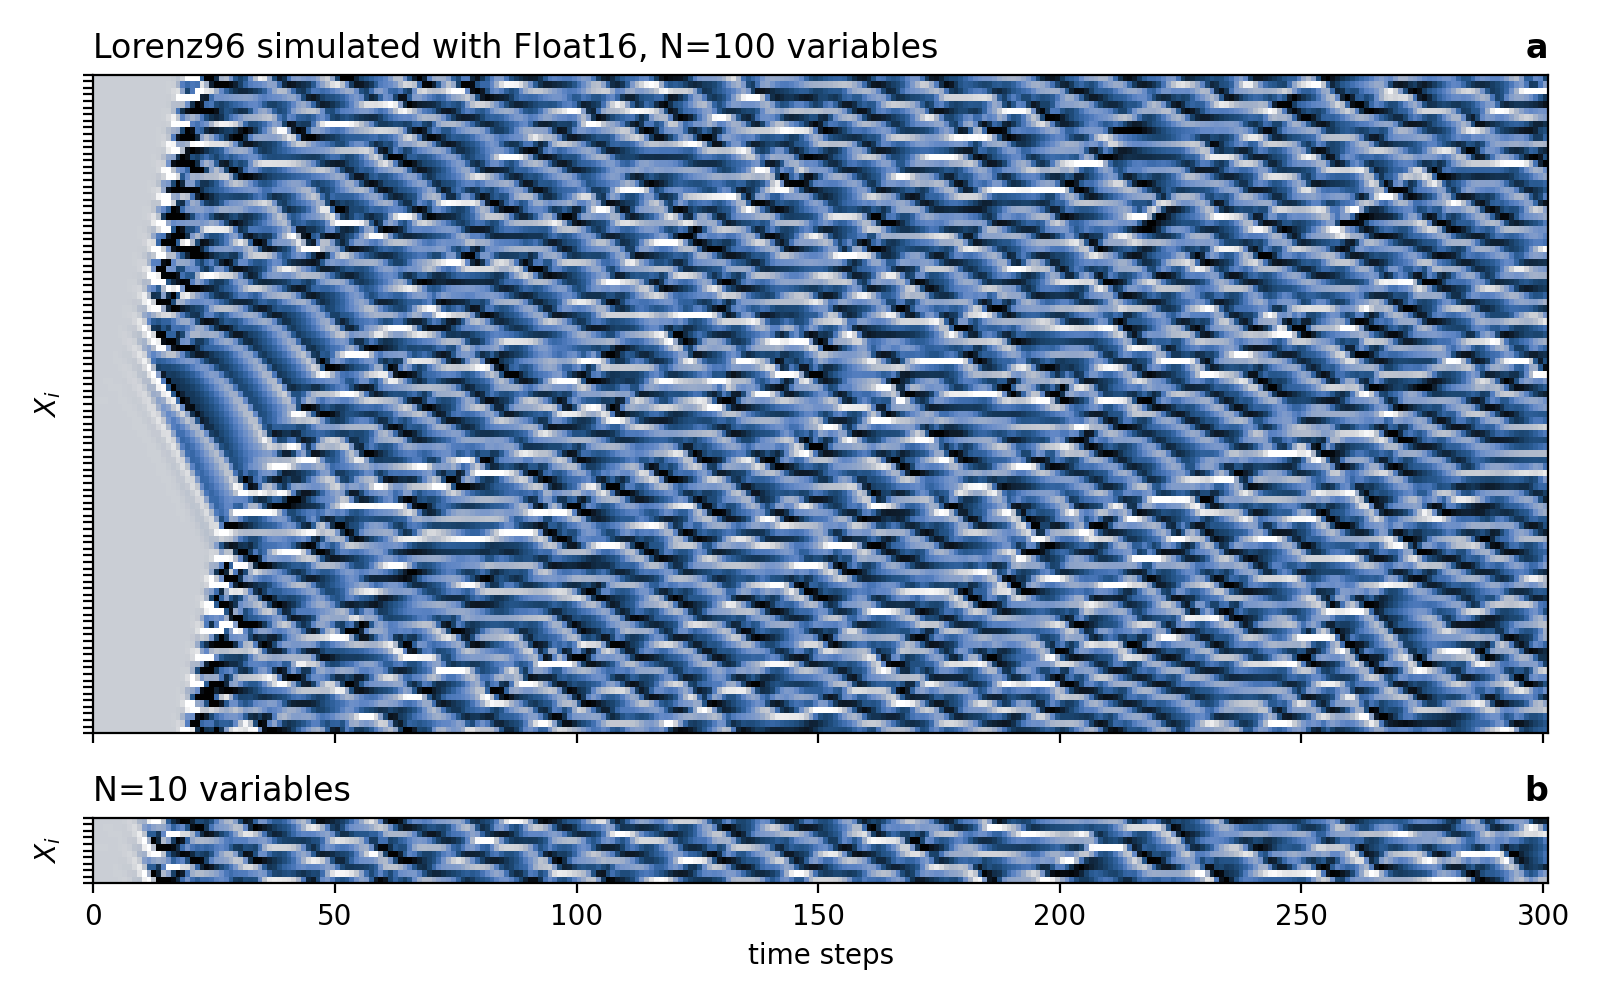
\includegraphics[width=1\textwidth]{Figures/orbits/hovmoeller.png}
	\caption{\textbf{The Lorenz 1996 system simulated with Float16 arithmetic. a}
	$100$ variables are used, starting from equilibrium with a small perturbation in $X_{50}$, and
	\textbf{b} $10$ variables starting with a small perturbation in $X_5$. Rectangles visible in shading
	represent individual variables and time step.}
	\label{fig:orbits_hovmoeller}
\end{figure}

\begin{figure}[tbhp]
	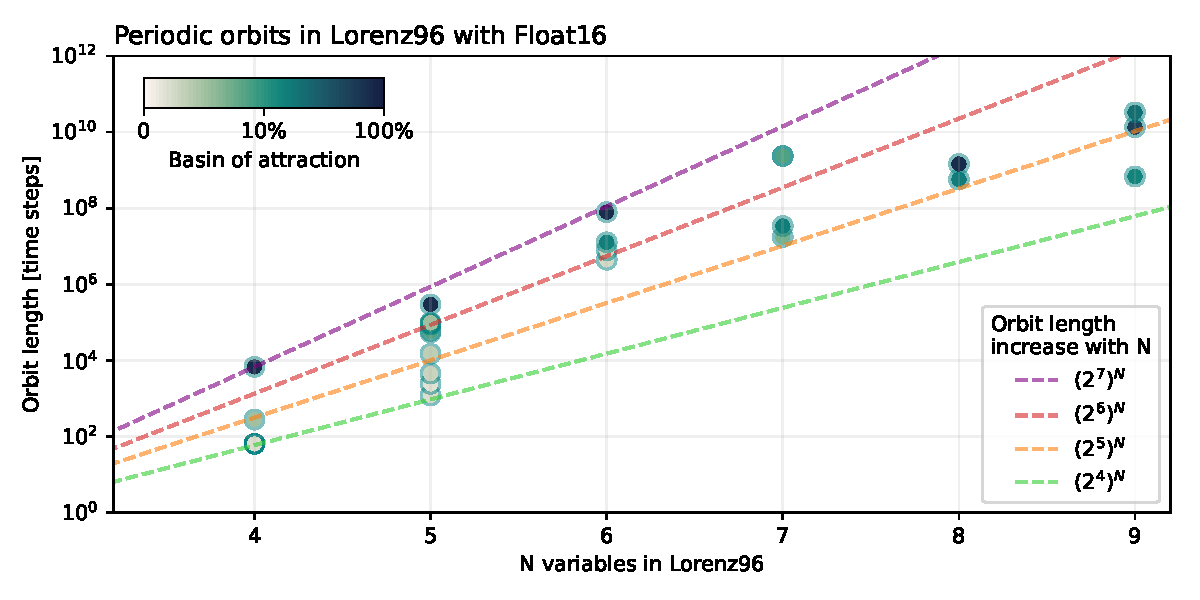
\includegraphics[width=1\textwidth]{Figures/orbits/L96_orbits.pdf}
	\caption{\textbf{Periodic orbits in Lorenz96 simulated with Float16 and an increasing number of
	variables.} Initial conditions are randomly taken from a spin-up simulation. Size of the basins of
	attraction (shading) correspond to the share of initial conditions that converge to the respective
	periodic orbit. Dashed lines provide an orientation for the exponential increase in orbit lengths
	with the number of variables.}
	\label{fig:L96_orbits}
\end{figure}

\begin{figure}[tbhp]
	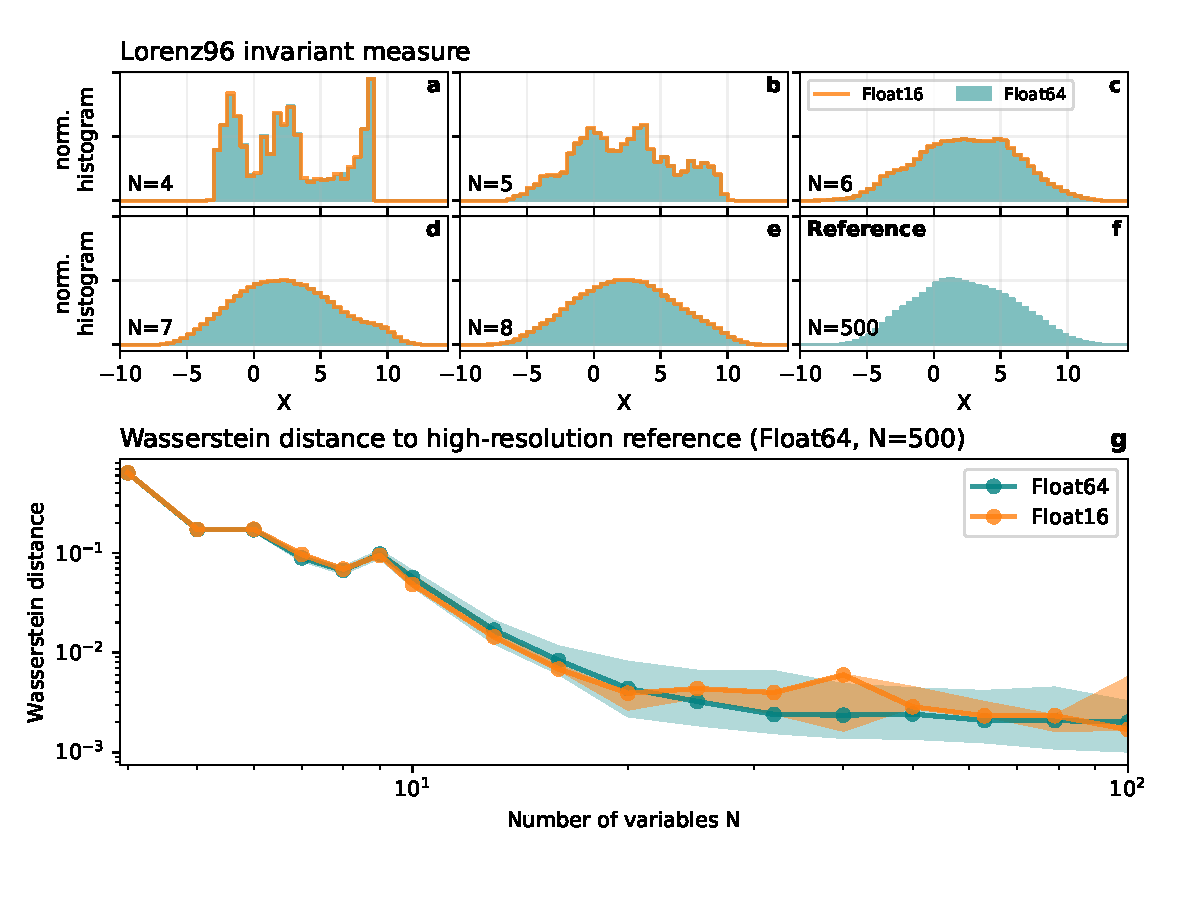
\includegraphics[width=1\textwidth]{Figures/orbits/L96_invmeasures.pdf}
	\caption{\textbf{Improvement of the simulated Lorenz 1996 invariant measure with increasing
	number of variables. a} The invariant measure of Lorenz 1996 simulated with 4 variables. Using
	Float16 or Float64 arithmetic yields a virtually identical invariant measure. b-e as a but with an
	increasing number of variables. f The reference invariant measure obtained from 500 variables
	using Float64 arithmetic. g The Wasserstein distance of the simulated Lorenz 1996 system with
	respect to the reference. Invariant measures are taken from all available variables, which are
	invariant due to periodic boundary conditions and spatially-independent forcing (see Eq. \ref{eq:L96}).
	Shadings in g represent the 5-95\% confidence interval and solid lines the median obtained from
	an ensemble simulation with 51 members starting from slightly perturbed random initial conditions.}
	\label{fig:L96_invmeasures}
\end{figure}

\section{Discussion}